
\documentclass[pdf]{beamer}

\mode<presentation>{}

\usetheme{CambridgeUS}

\usepackage[utf8]{inputenc}
\usepackage{tikz}
\usetikzlibrary{positioning}
\usetikzlibrary{calc}

\title{Tower Defense}
\author{Alexis Laouar, R\'emi Oudin, K\'evin Le Run}

\begin{document}

\begin{frame}
  \titlepage
\end{frame}

\begin{frame}
  \frametitle{Plan}
  \tableofcontents
\end{frame}

\section{Architecture}

\subsection{MVC}

\begin{frame}
  \frametitle{Mod\`ele Vue Contr\^oleur}
  \begin{figure}[h]
    \centering
    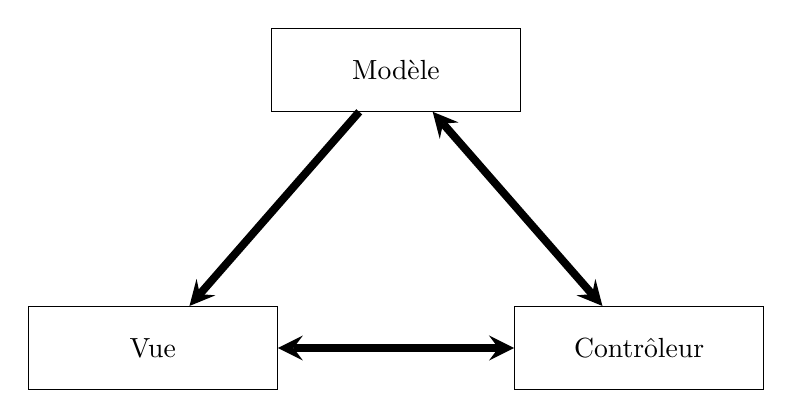
\begin{tikzpicture}[
      elementblock/.style={draw,rectangle,minimum height=3em, minimum width=9em},
      node distance=3cm]
      % Blocks
      \node[elementblock]                                     (view)      {Vue};
      \node[elementblock,right=of view]                       (controller){Contr\^oleur};
      \node[elementblock,above=of {$(view)!0.5!(controller)$}](model)     {Mod\`ele};

      % Arrows
      \draw[         -{stealth},thick,line width=0.1cm] (model) edge (view);
      \draw[{stealth}-{stealth},thick,line width=0.1cm] (model) edge (controller) (controller) edge (view);

    \end{tikzpicture}
    \caption{Modèle-Vue-Contrôleur}
  \end{figure}
\end{frame}

\subsection{Design Patterns}

\begin{frame}
  \frametitle{Type Object}
  \begin{tikzpicture}
    
  \end{tikzpicture}
\end{frame}

\section{Difficult\'es rencontr\'ees}

\section{Conclusion}

\end{document}